%%=============================================================================
%% Implementatie
%%=============================================================================

\chapter{Technische uitwerking}%
\label{ch:implementatie}

In dit hoofdstuk wordt de technische implementatie van het prototype besproken.
De applicatie werd ontwikkeld als een client-side proof-of-concept, met als doel
een mobielvriendelijke gebruikerservaring te bieden zonder afhankelijkheid van een backend.

\section{Technologiestack}

Het prototype werd ontwikkeld met volgende technologieën:

\begin{itemize}
  \item \textbf{React} als front-end framework voor componentgebaseerde ontwikkeling;
  \item \textbf{TypeScript} voor typeveiligheid en betere onderhoudbaarheid;
  \item \textbf{Vite} als build tool voor snelle development en bundling;
  \item \textbf{pnpm} als package manager voor dependencybeheer;
  \item \textbf{Tailwind CSS} voor styling en consistente UI-componenten;
  \item \textbf{Lucide React} voor iconografie.
\end{itemize}

Deze stack werd gekozen omdat ze snel prototyping mogelijk maakt en goed aansluit bij moderne
webdevelopment-praktijken.

\section{Architectuur}

Aangezien de applicatie volledig client-side werkt, is de architectuur relatief eenvoudig.
De kern bestaat uit React componenten die via state management en lokale opslag met elkaar communiceren.

\begin{figure}[h]
\centering
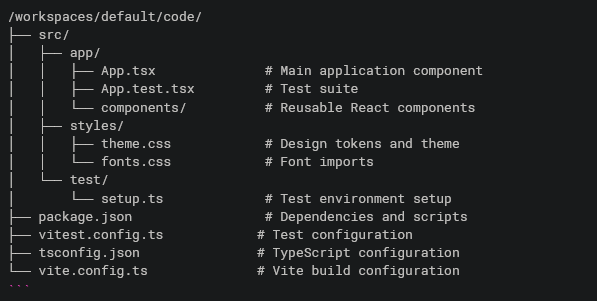
\includegraphics[width=0.8\linewidth]{architectuur.png}
\caption[Architectuur van het prototype]{Globale architectuur van de applicatie. De applicatie draait volledig client-side en gebruikt lokale opslag voor het bewaren van taken en gebruikersvoortgang.}
\label{fig:architectuur}
\end{figure}

\textbf{[AANVULLEN: maak een eenvoudig blokdiagram en exporteer als architectuur.png]}

\section{Dataopslag}

Omdat het prototype geen backend bevat, wordt data lokaal opgeslagen.
Hiervoor kan gebruik gemaakt worden van bijvoorbeeld \texttt{localStorage} of \texttt{IndexedDB}.
Dit laat toe om taken en gebruikersvoortgang tijdelijk te bewaren zonder server.

\subsection{Structuur van taakdata}

Elke taak bevat minstens:
\begin{itemize}
  \item een unieke identifier;
  \item een titel;
  \item een datum (geplande dag);
  \item een status (voltooid of niet);
  \item optioneel een beschrijving.
\end{itemize}

\section{Navigatie en componentstructuur}

De applicatie is opgebouwd uit verschillende pagina’s/schermen:
\begin{itemize}
  \item Dashboard of dagoverzicht;
  \item Takenbeheer;
  \item Reward/voortgangsoverzicht;
  \item Profielpagina;
  \item Instellingen.
\end{itemize}

Deze schermen zijn als afzonderlijke componenten geïmplementeerd en hergebruiken gedeelde UI-elementen.

\section{Voorbeeld van codefragment}

Onderstaand fragment toont een vereenvoudigd voorbeeld van hoe taken worden toegevoegd.

\begin{listing}[ht]
\caption[Voorbeeld: toevoegen van een taak]{Vereenvoudigd voorbeeld van een functie die een taak toevoegt aan de lokale taaklijst.}
\label{lst:add-task}
\begin{minted}{typescript}
const addTask = (title: string, date: string) => {
  const newTask = {
    id: crypto.randomUUID(),
    title,
    date,
    completed: false
  };

  setTasks((prev) => [...prev, newTask]);
};
\end{minted}
\end{listing}

\section{Beperkingen van de implementatie}

De keuze om geen backend te gebruiken zorgt ervoor dat:
\begin{itemize}
  \item data niet gesynchroniseerd wordt tussen toestellen;
  \item er geen login-systeem is;
  \item gegevens verloren kunnen gaan bij het wissen van browserdata.
\end{itemize}

Deze beperkingen zijn aanvaardbaar binnen de scope van een proof-of-concept, maar zouden in een productieomgeving
moeten opgelost worden via een backend en een degelijk gebruikersbeheer.